
% !TEX root = DesignDocument.tex

\chapter{Design  and Implementation}
This section is used to describe the design details for each of the major components 
in the system.   The major components include: Parse for our database, Sinch for messaging, 
and native APKs (Google and Apple) for maps.   

(TODO) Citations look like~\cite{Choset:2005:PRM, arkin2009governing, lavalle2006}  and~\cite{wiki:asimo,lumelsky:1987, nolfi2000evolutionary}.  These are done automatically.  Just fill in the database {\tt designrefs.bib} using the same field structure as the other entries.  Then pdflatex the document, bibtex the document and pdflatex twice again.  The first pdflatex creates requests for bibliography entries.
The bibtex extracts and formats the requested entries.  The next pdflatex puts them in order and assigns labels.  The final pdflatex replaces references in the text with the assigned labels.
The bibliography is automatically constructed.  
 
 \section{Architecture and System Design}
 This is section will detail the overall system design and general architecture of Crowd Control. The software was designed in such a way that minimizes dependency from third-party services such as Sinch and Parse.  It does this by abstracting everything using an extra layer of models.  The extra models stop the third party calls from being visible in the main activities in Android as well as the view logic in iOS.
 
 \subsection{Design Selection}
Sprint 1 was centered around designing of the database schema and the general system architecture. Bowtaps produced various high-level designs on both the front-end and back-end of the system that were deeply inspected before deciding on our current implementation. Later, the architecture evolved as the year progressed, and there were changes to the overall UX as well as how the apps themselves retrieved the data from parse. In addition, the database schema was changed over winter break to include the knowledge we learned over the first sprint. These changes still persist though our current product.

\subsubsection{Early Design Ideas}
The original database design for Crowd Control consisted of three tables with associated data. Though this design provided a good sense of direction and foundation to build upon, it eventually would need to expand as Crowd Control's feature set expanded. See Figure~\ref{EarlyDBSchema} below.

	\begin{figure}[tbh]
	\begin{center}
	\fbox{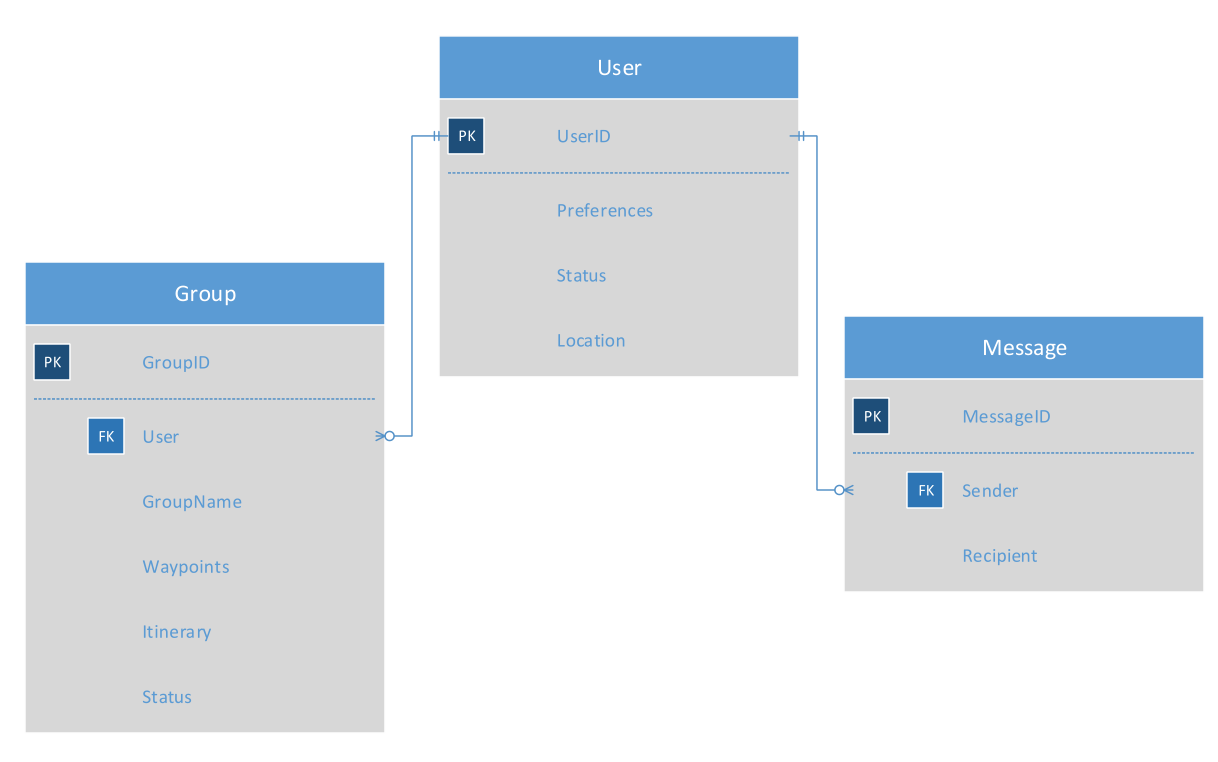
\includegraphics[scale=.5]{Additional/DesignPictures/CC_dbSchema1.PNG}}
	\end{center}
	\caption{Early database schema. \label{EarlyDBSchema}}
	\end{figure}

Another caveat to this design is the failure to differentiate between public and private user data. In Crowd Control, each user has data that is private to that user, such as their email and password. However, there is also a set of public data that can be viewed by other users, such as their display name or their location. This iteration of the schema only has one user entity, that stores their information. A small lack of understanding about Parse's no-SQL implementation lead us to improperly design our entities in this way. It was later deemed that this separation between front-facing and hidden user data entities was necessary in terms of ease-of-access and information privacy.

\subsubsection{Improvements to Early Designs}
In reflection of the shortcomings of the first design iteration, the database schema was restructured to better fit Crowd Control's needs. The current design consists of eight data tables,  shown in Figure~\ref{MidDBSchema} below. More entities were added to the overall schema. One such addition was a ``CCUser'' table to hold the public data associated with a user. It is important to note that the ``User'' table was left to hold a user's private data. Those changes and some additions resulted in the below schema. 

	\begin{figure}[tbh!]
	\begin{center}
	\fbox{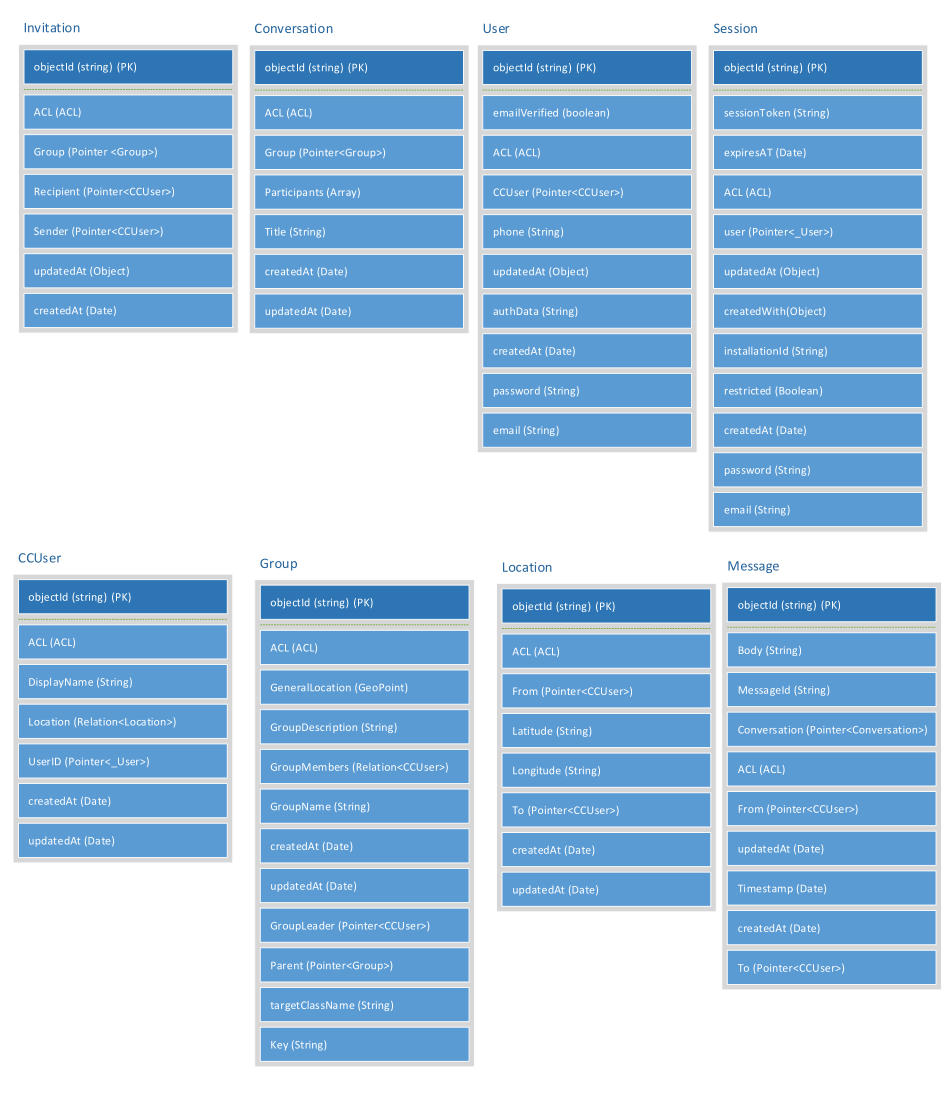
\includegraphics[scale=.65]{Additional/DesignPictures/CC_dbSchema2.PNG}}
	\end{center}
	\caption{Improved database schema. \label{MidDBSchema}}
	\end{figure}

 \subsection{Data Structures and Algorithms}
 By developing Crowd Control in the Android Studio environment, all the data structures available to Java are available to the project itself. That being said, there are no particularly noteworthy structures or algorithms that need to be expound upon, but there are class hierarchies that will be explained in later detail in this chapter.
 
 \subsection{Data Flow}
 TODO: Create Data Flow diagram of overall process
 
 
 \subsection{Communications}
 One of the core features to the Crowd Control app is communication amongst its users. To achieve this, some third-party services are used, which in turn communicate data between users. If a user wishes to send another user a message, that message is sent to the Parse back-end, and delivered to the recipient via the Sinch service. The basic communication overview is outlined below in Figure ~\ref{CommFlow}.
 
  	\begin{figure}[tbh]
	\begin{center}
	\fbox{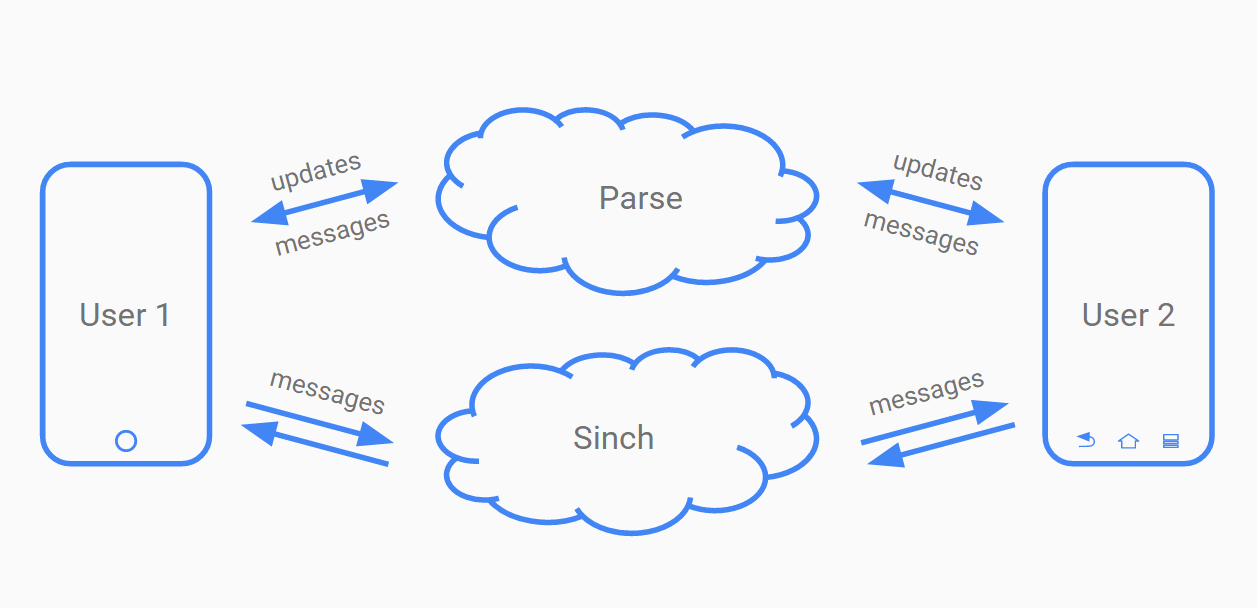
\includegraphics[scale=.5]{Additional/DesignPictures/CommFlow.PNG}}
	\end{center}
	\caption{Communication flow diagram. \label{CommFlow}}
	\end{figure}
 
 In addition to message-passing, various other data is being transferred from the users' devices. One such example is GPS data. Upon retrieval of a user's location, that value is stored in Parse, and able to be fetched by any group member that wishes to see that location. 

 \subsection{Classes}
 
 	\subsubsection{Sign up and Log in Classes}
 	Everything starts with the WelcomeActivity.java class. This initial activity checks if the user has logged in or not by looking against its local Parse database. If a user has logged in or signed up it will be stored in the local Parse database.
 	
 	The SignupActivity.java is next on the list. It allows a user to sign into parse, it was created using the Android log-in/sign-up template. From here a user can access a Facebook log-in page and a Twitter log-in page. Additionally the class, LoginActivity.java allows the user to log into a registered email account.
 	
 	For either of the previous paths, the next class the user will enter is GroupJoinActivity.java.
 	\subsubsection{Menu Classes}
 	The menu can be accessed from the top right of the app after a user has either logged in or created an account. The code for the creation of the menu can be found in GroupJoinActivity.java (for a basic menu) and in GroupInfoFragment.java (which can be basic or a leader menu). 
 	
 	The classes connected to the menu include: SettingsActivity.java, NotificationActivity.java and InviteNavigationActivity.java.  The SettingsActivity.java class allows a user to log out and return to the SignUpActivity.java class, as well as see what group they are in, and gives the user the ability to change their user name. The NotificationActivity.java allows the user to access all their in app notifications. The InviteNavigationActivity.java will be discussed later because it is only accessible if the user is a leader of a group.
 	\subsubsection{Initial Tab Class}
 	After a user has joined a group in the class GroupJoinActivity.java, they will reach GroupNavigationActivity.java. This activity is in charge of displaying the four Fragment class: EventFragment.java, GroupInfoFragment.java, MessagingFragment.java, and MapFragment.java. It is the main UX for the user for the duration of a group.
 	
 	The EventFragment.java is not implemented and is no longer accessible in the app.
 	\subsubsection{Group Management Classes}
 	The GroupInfoFragment.java class is the main class for group management tools. This class allows a leader of a group to kick a member or promote a new leader. This class also holds the code for the group menu. The group menu also allows the user to change the group name.
 	
 	Other group management classes can be accessed though the menu for group leaders. These classes include: InviteNavigationActivity.java, InviteConfirmFragment.java, and InviteSearchFragment.java. The InviteNavicationgActivity.java class is much like the GroupNavigationActivity.java class. It is a tab system holding the other two classes. The InviteSearchFragment.java allows the leader to search for other users they wish to add to the group. It creates a group list that is given to the InviteConfirmFragment.java class. Here the leader can make sure that these are the people that he/she want to invite and completes the process.
 	\subsubsection{Location Classes}
 	Location functionality took place in three major locations: the GoogleLocationListener.java file in the ``location'' folder, the MapFragment.java file in the ``com.bowtaps.crowdcontrol'' folder, and the GroupService.java file in that same folder. 
 	
 	The map fragment serves as the controller for the fragment\_map.xml layout file. Since this is a fragment, in contrast to an activity, it must be nested in an activity class. The MapFragment.java class is nested inside the actual tab adapter. 
 	
 	The two other files work together to call methods to update and store location data when desired. This functionality is done via cloud code in order to carry these tasks out asynchronously. In short, the listeners on the service communicate with the cloud code, which carries out the desired functions, and reports it back to the listener. The data is then updated on the model, for the user and for the group members.
 	\subsubsection{Messaging Classes}
 Messaging consisted of a three major classes. These class include MessageService.java, MessageAdapter.java, and MessagingFragment.java. The MessagingFragment.java class is part of the tab system found in the InviteNavigationActivity.java. This way it can be a key component to the flow of groups. The MessageAdapter.java is a helping class. Its sole purpose is to modify message objects into views so that they can be displayed in the MessagingFragment. The MessageService.java handles our apps connection to Sinch. It's a stand alone service that sends and receives messages with other Sinch servers. Without this service the app wouldn't be able to listen for new messages. Finally, our overarching server, that handles all the updates for data in the database, also handles storing conversations. Each group has its own conversation in the database, that way the conversation can be loaded into the MessageService.java class so that they can be loaded for new members or if something happens to an existing members local copy.

I explicitly want to note that the messaging service and many of the GUI elements were taken from a GitHub repository owned by Sinch \cite{sinch:github}. This repository gives full permission for commercial use ~\cite{Choset: License, https://github.com/sinch/android-messaging-tutorial/blob/master/LICENSE}.

	\subsubsection{Miscellaneous Classes}
	There were a few classes not explained from the ones listed above including: CrowdControlApplication.java, GroupJoinActivity.java, and GroupService.java.
	
	The CrowdControlApplication.java is the very first class that initializes the app on launch, it loads up any locally stored data as well as holds some global classes so that other activities can access them.
	
	The GroupJoinActivity.java class loads in the groups for the user to select a group. It also holds a basic menu for a user to get to their own user related info. This class also uses the GroupModelAdapter.java class. This is used to change group models loaded in from Parse into objects that can be displayed in a list.
	
	The SimpleTabsAdapter.java is used to create views to hold multiple fragments in one activity. This used used in GroupNavigationActivity.java and in InviteNavigationActivity.java.

 \subsection{UML}
 Below in \ref{UseCaseUML}is a high-level use case UML diagram that shows basic user functionality of the Crowd Control application. The light-blue nodes are reserved for group leaders only, but the green colored nodes are available to all users. Once a group leader promotes another user to become the new group leader, the previous leader simply becomes a group member and loses their leader privileges. Of course, after creating a group, one must have group members in order to kick or promote members, as well as message or locate other members in the first place.
 
 	\begin{figure}[tbh!]
	\begin{center}
	\fbox{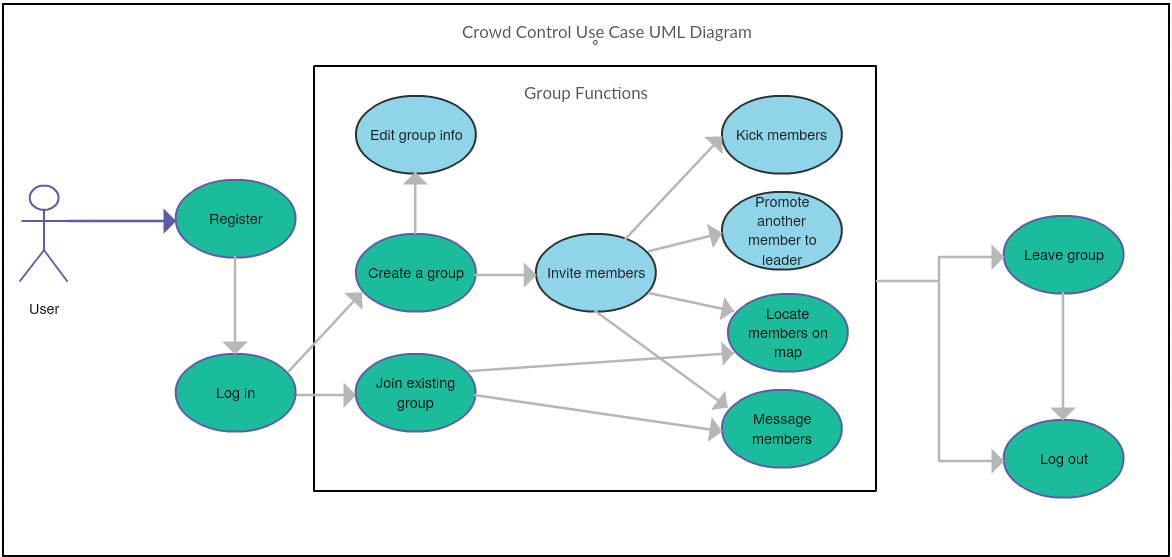
\includegraphics[scale=.55]{Additional/DesignPictures/Use-Case-UML.PNG}}
	\end{center}
	\caption{Use Case Diagram in UML. \label{UseCaseUML}}
	\end{figure}
 
 \subsection{GUI}
 Designing the user interface of a mobile application has many unique challenges, all of which influence design decisions. In order to present users with a satisfying and intuitive experience, it is suggested to follow material design pattern aspects such as using Floating Action Buttons (FABs), and simply adhering to a more unified experience that can be found across multiple new applications on many platforms. With that in mind, we also focused on keeping the overall design very clean and free from clutter.
 
 Another influence on our design choices, was the integration of Google Services in Crowd Control. Since Google's components currently follow a material design approach, we chose to do so as well to ensure a consistent experience when a user interacts with one of their interfaces.
 
 Lastly, Crowd Control was designed to look similar to users, regardless of their platform; an Android user should have a very similar interface, compared to that of an iOS user, and vice versa. By choosing elements from each platform's respective layout styles, we are also able to create a design that conforms to the guidelines set by the device or platform itself. Ultimately, our design choices ensure that users have a consistent user experience, independent of their platform or their device.
 
 \subsection{MVC}
 
 \subsubsection{Introduction}
 MVC, or ``model-view-controller'' is a design pattern used widely in mobile applications to separate an application's core functionalities. \begin{itemize}
  \item Model - Model represents an object to carry or store data. It can also have logic to update a controller if its data changes.
  \item View - Views represent the visualization of the data that model contains, such as a screen or an activity in Android. These are represented as a layout generally.
  \item Controller - Controllers act on both the model and the views. They control the data flow into model objects and updates the view whenever data changes. It maintains a separation between the view and the model.
\end{itemize}
 
 
 \subsubsection{Models}
In Android, the models are a collection of model classes, such as the GroupModel and the UserModel, as well as other various storage classes. They can be found in a ``models'' folder at ``\textasciitilde /CrowdControl/app/src/main/java/com/bowtaps/crowdcontrol/model/'', shown below in \ref{ModelFolder}:

	\begin{figure}[tbh!]
	\begin{center}
	\fbox{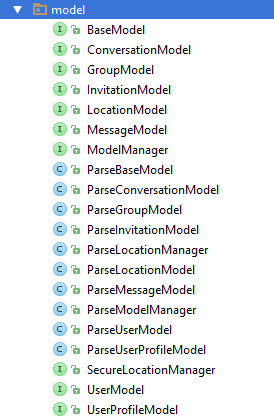
\includegraphics[scale=.85]{Additional/DesignPictures/FD-model-folder.PNG}}
	\end{center}
	\caption{Model classes in the ``model'' folder of the project. \label{ModelFolder}}
	\end{figure}

 Our models were designed to be abstracted away from our third party software in order to keep API-specific code of the activities. In this way, one could implement a different back-end service instead of Parse with minimal refactoring. We have several models that keep track of local data and keep up to date with our Parse database using a service. These models can be accessed by controllers. This is initialized CrowdControlApplication.java, which is the global main class of the app, serving as the application's entry point.
 
 \subsubsection{Controllers}
 Each activity file is a controller, and is responsible for calling functions from the models to either change data in the database, or to update the data in the layouts; it facilitates information between the models and the views. Each activity has one layout in general. These layouts take place in the form of XML files, and thus their tags are specific to the Android Studio/Java environment. Controller files can be found at ``\textasciitilde /CrowdControl/app/src/main/java/com/bowtaps/crowdcontrol/'', shown below in \ref{ControllersFolder}:
 
 	\begin{figure}[tbh!]
	\begin{center}
	\fbox{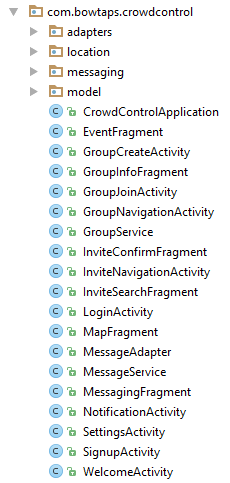
\includegraphics[scale=.85]{Additional/DesignPictures/FD-controller-folder.PNG}}
	\end{center}
	\caption{Model classes in the ``model'' folder of the project. \label{ControllersFolder}}
	\end{figure}
 
 \subsubsection{Views}
 As stated, views typically take the form of XML files in the Crowd Control project. These files contain no business logic, and simply contain layout information that pertains to the appearance and attributes of the page itself. These layouts are constructed via the Android Studio layout designer, then edited to tailor to our specific needs. Views can be found at ``\textasciitilde /CrowdControl/app/src/main/res/layout/'', shown below in \ref{ViewsFolder}:
 
	\begin{figure}[tbh!]
	\begin{center}
	\fbox{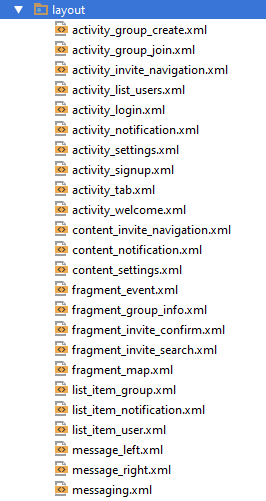
\includegraphics[scale=.85]{Additional/DesignPictures/FD-view-folder.PNG}}
	\end{center}
	\caption{Model classes in the ``model'' folder of the project. \label{ViewsFolder}}
	\end{figure}

\section{Group Messaging }

\subsection{Technologies  Used}
\begin{itemize}
  \item Parse - back-end database tool.
  \item Sinch - back-end messaging tool.
\end{itemize}

\subsection{Component  Overview}
\begin{itemize}
  \item Send/receive messages to/from group members (many-to-many)
  \item Store messages in Parse (data persistence)
  \item Message transfer service is independent of carrier/device/platform
\end{itemize} 

\subsection{Phase Overview}
%TODO: Fix citations. The .bib file is set up correctly, and we are properly accessing the .bib sub-structure, but it is either not being displayed correctly. Perhaps incorrect compilation option? Syntax inconsistency?

%Group Messaging uses Sinch as a back-end. It allows are users to send a message to every other user in their group. We have modified code from this repository to do group messaging ~\cite{Choset: sinch/android-messaging-tutorial, https://github.com/sinch/android-messaging-tutorial}. This repository gives full permission for commercial use ~\cite{Choset: License, https://github.com/sinch/android-messaging-tutorial/blob/master/LICENSE}. 

\begin{description}
  \item [Phase 1] Construct message containers and begin Sinch integration
  \item [Phase 2] Construct messaging activity and view to encapsulate functionality
  \item [Phase 3] Construct conversation containers to associate groups of messages
  \item [Phase 4] Implement many-to-many message passing/broadcasting through Sinch delivery
  \item [Phase 5] Store associated messages inside conversations, both on Parse, as well as caching locally on the user device
\end{description}

\subsection{Architecture Diagram}
It is important to build and maintain an architecture diagram.  However, it may 
be that a component is best described visually with a data flow diagram. 

\subsection{Data Flow Diagram}

	\begin{figure}[tbh!]
	\begin{center}
	\fbox{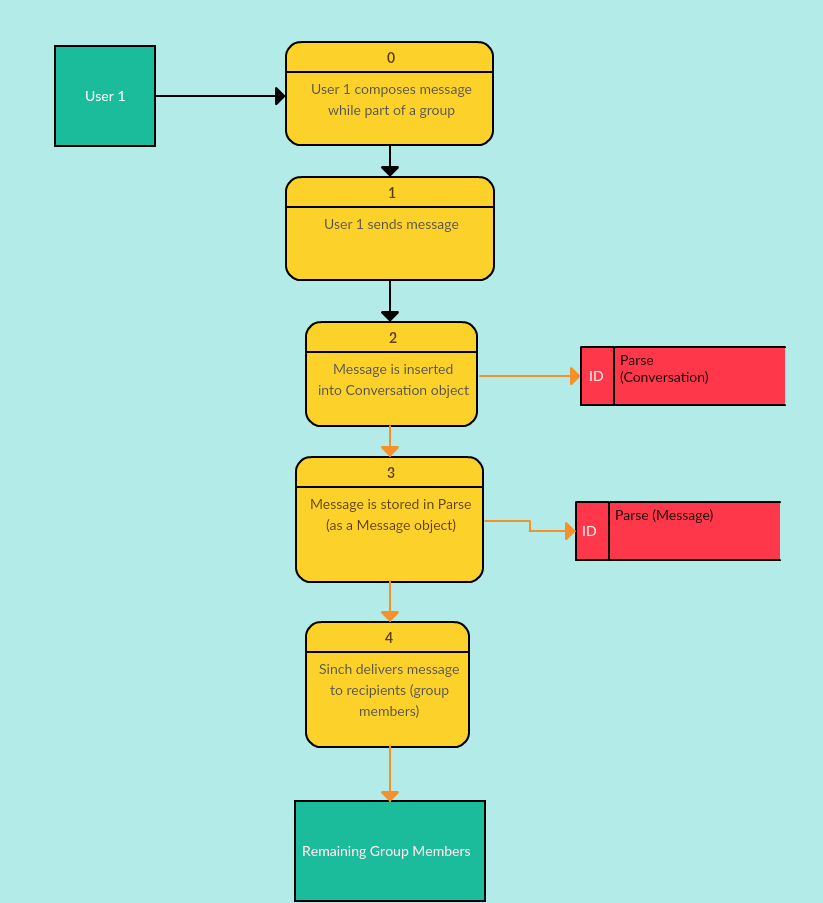
\includegraphics[scale=.60]{Additional/DesignPictures/MessagingDataFlow.PNG}}
	\end{center}
	\caption{Messaging data flow diagram. \label{MessagingDataFlow}}
	\end{figure}

\subsection{Design Details}
Messaging interfaces with the user though the MessagingFragment.java class. This class uses the MessageAdapter.java class to take the data from the MessageService.java class, and display it to the user. The MessagingFragment.java class also allows the user to send messages though the MessageService.java class to all other members in the group.
The MessagingFragment.java class relies on the apps overarching service to keep its messages stored in Parse. This allows the class to load a conversation (group object that holds messages) into view for the user, if that user doesn't have them or loses their local copy.

\section{Location Tracking }

\subsection{Technologies  Used}
\begin{itemize}
  \item Google Play Services / Apple Map Features
  \item Parse
\end{itemize}

\subsection{Component  Overview}
\begin{itemize}
  \item Track all group members in a map fragment
  \item Homing functionality on the user's location pin
  \item Sync group locations automatically (interval-based) and manually (on button-press)
\end{itemize}

\subsection{Phase Overview}
\begin{description}
  \item [Phase 1] Construct location containers and begin location services integration
  \item [Phase 2] Construct map fragment, buttons for future homing/syncing functionality
  \item [Phase 3] Implement homing and location syncing features, as well as interval-based location syncing
  \item [Phase 4] Extract location update functionality from client, place into cloud-based service for better (faster) asynchronous user experience
\end{description}

\subsection{ Architecture  Diagram}
It is important to build and maintain an architecture diagram.  However, it may 
be that a component is best described visually with a data flow diagram. 

\subsection{Data Flow Diagram}
It is important to build and maintain a data flow diagram.  However, it may be 
that a component is best described visually with an architecture diagram. 


\subsection{Design Details}
This is where the details are presented and may contain subsections. 

\section{Group Management }

\subsection{Technologies  Used}
\begin{itemize}
  \item Parse
\end{itemize}

\subsection{Component  Overview}
\begin{itemize}
  \item Store group members in a group
  \item Incorporate a party leader to manage the group (has special privileges)
  \item Create a group with specific attributes that can be changed by the leader
\end{itemize}

\subsection{Phase Overview}
\begin{description}
  \item [Phase 1] Construct model layer and base model classes to communicate with Parse and store data application-side
  \item [Phase 2] Allow users to create or join groups, manage group members that join and create groups
  \item [Phase 3] Add Group Leader functionality to manage group (kick/promote members, edit description, etc)
  \item [Phase 4] Begin design/integration of messaging components for group management
\end{description}
\subsection{ Architecture  Diagram}
\begin{figure}[tbh!]
	\begin{center}
	\fbox{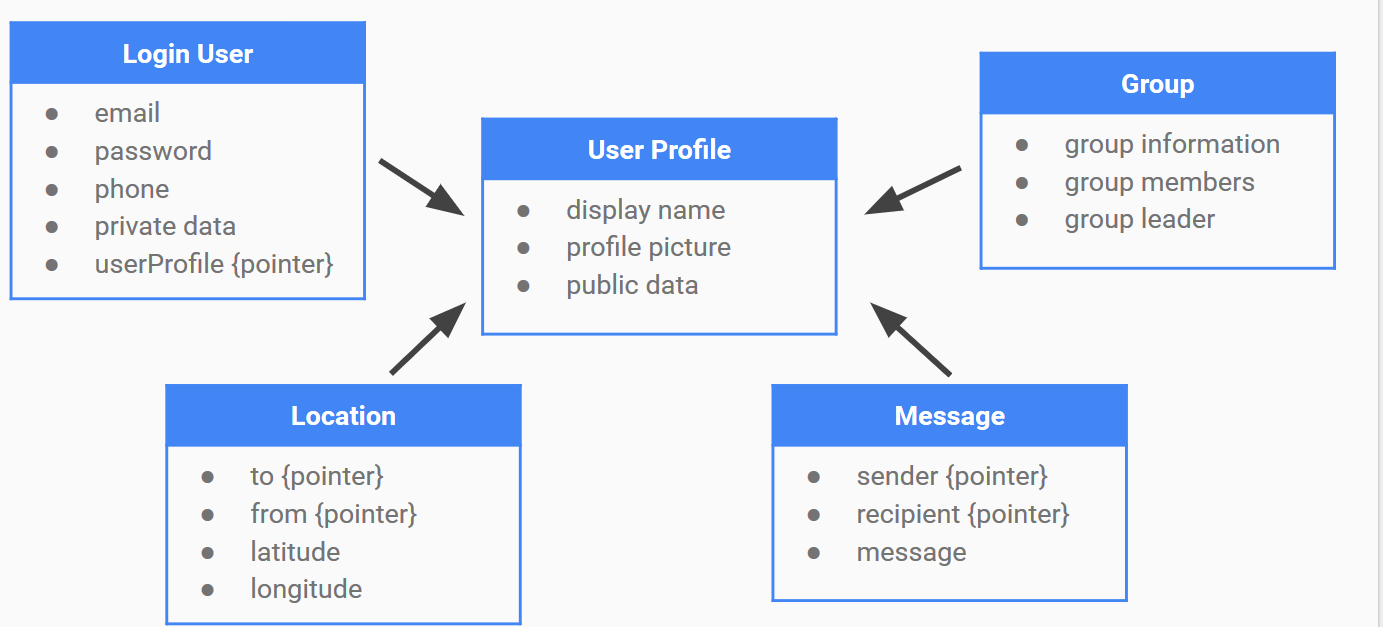
\includegraphics[scale=.60]{Additional/DesignPictures/ParseArch.PNG}}
	\end{center}
	\caption{Architecutre of Group \label{ArchitecutreofGroup}}
	\end{figure}


\subsection{Data Flow Diagram}
See Figure~\ref{ArchitecutreofGroup}


\subsection{Design Details}
This is where the details are presented and may contain subsections. 


